En regardant rapidement les données fournies dans le fichier \emph{train.txt}, on peut voir que les échanges de textos sont très courts. Également, il y a beaucoup d'\emph{emojis} et de binettes créés à partir de caractères spéciaux (ex: :), :D, :(, :-)).

On peut regarder le nombre de textes avec la présence d'au moins un emoji particulier selon chaque classe pour voir si ceux-ci semblent être beaucoup plus présents dans une classe ou une autre. Les résultats obtenus pour quelques emojis testés se trouvent dans la figure ....

% Please add the following required packages to your document preamble:
% \usepackage{booktabs}
\begin{table}[]
	\centering
	\caption{My caption}
	\label{my-label}
	\begin{tabular}{@{}lllll@{}}
		\toprule
		Emoji testé & Angry & Happy & Sad & Others \\ \midrule
		❤           & 8     & 31    & 13  & 41     \\
		💔          & 2     & 0     & 64  & 3      \\
		😍          & 10    & 88    & 10  & 92     \\
		😞          & 15    & 1     & 282 & 15     \\
		😂          & 59    & 989   & 49  & 197    \\
		😡          & 156   & 6     & 18  & 10     \\ \bottomrule
	\end{tabular}
\end{table}

%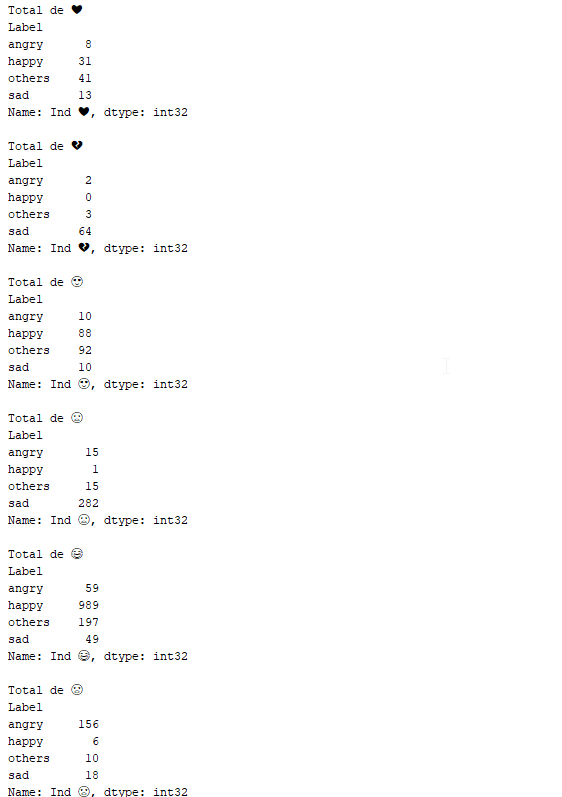
\includegraphics[width=\linewidth,height=15cm,keepaspectratio]{images/analyse_emojis}

À première vue, les emojis semblent avoir un impact important. Par exemple, le coeur brisé et le bonhomme triste sont souvent utilisés dans des échanges de textos tristes alors que celui qui fait un sourire est utilisé pour les échanges neutres ou joyeux. Il semble donc pertinent de convertir tous les emojis en texte pour les traiter avec un objet de compte de mots.

On peut également tenter de repérer les binettes créés à partir de caractères spéciaux. Pour parvenir à les identifier, on peut utiliser une expression régulière qui identifie les séries de 2 à 6 caractères spéciaux:
\begin{verbatim}
reg ex : [^\w\s\d]{2,6}
\end{verbatim}

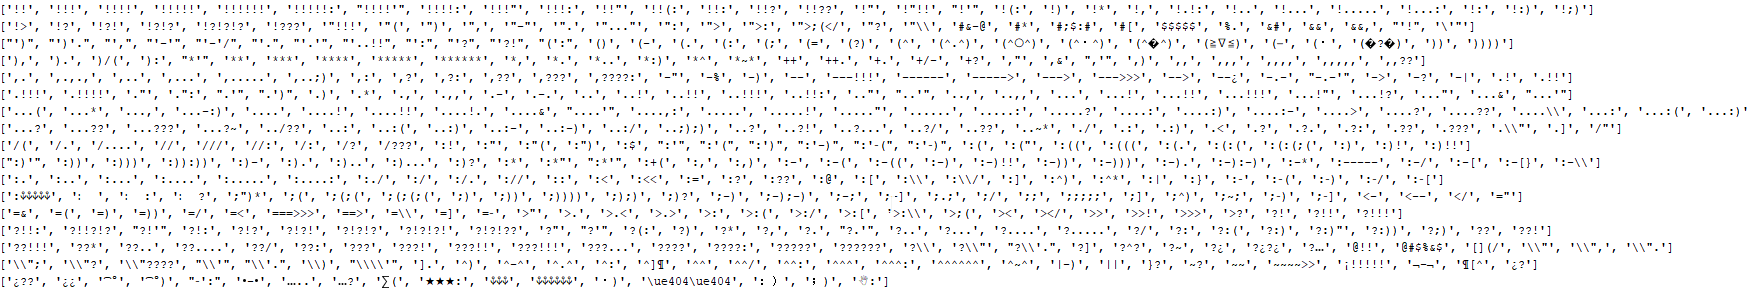
\includegraphics[width=\linewidth,height=7cm]{images/analyse_list_car_speciaux}

À partir de cela, on peut tenter d'identifier toutes les chaînes qui semblent intéressantes de façon manuelle. Voici une liste des plus intéressantes: 

\begin{figure}[h!] %h: place figure here if possible, t: top, b:bottom, !:over-ride default placement
	\begin{minipage}[b]{0.3\textwidth}
		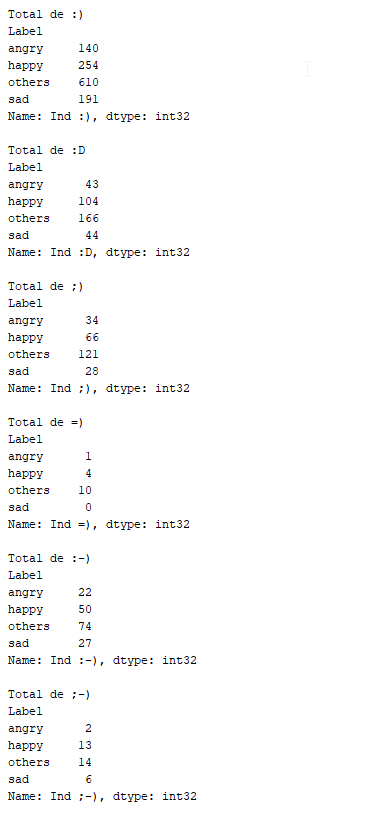
\includegraphics[width=\textwidth,height=14cm]{images/analyse_emojis_car_pos}
	\end{minipage}
	\hfill
	\begin{minipage}[b]{0.3\textwidth}
		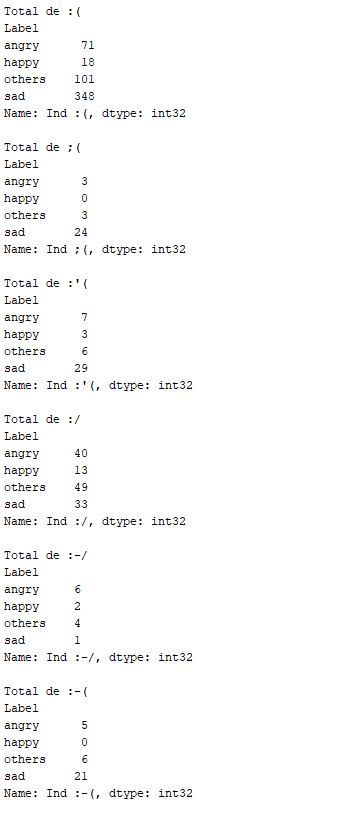
\includegraphics[width=\textwidth,height=14cm]{images/analyse_emojis_car_neg}
	\end{minipage}
	\hfill
	\begin{minipage}[b]{0.3\textwidth}
		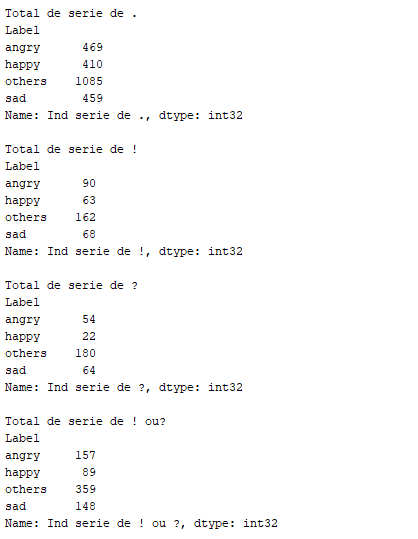
\includegraphics[width=\textwidth,height=14cm]{images/analyse_car_ponctuation}
	\end{minipage}
\end{figure}

On peut voir que les smileys qui ont une apparence plus joyeuse (ex: :), :D) sont souvent utilisés dans des textos joyeux ou autres. Pour ce qui est de ceux avec une apparence triste, on remarque qu'ils sont souvent dans les textos tristes et parfois ceux fâchés.

On peut également analyser la ponctuation, plus particulièrement une série de 3 signes de ponctuation et plus (ex: ..., !!!!!, ????, ?!?!??!). Les séries de points ne semblent pas particulièrement être plus présent dans une classe particulière. Pour ce qui est des séries de ! ou ?, on remarque qu'elles sont plus présentes dans les textos fâchés et triste.

On peut également s'attarder au pourcentage de lettres en majuscule dans un texto, ainsi que le score de sentiment, le nombre de mots positifs et négatifs. Voici la liste du nombre moyen de ces valeurs pour chaque classe:

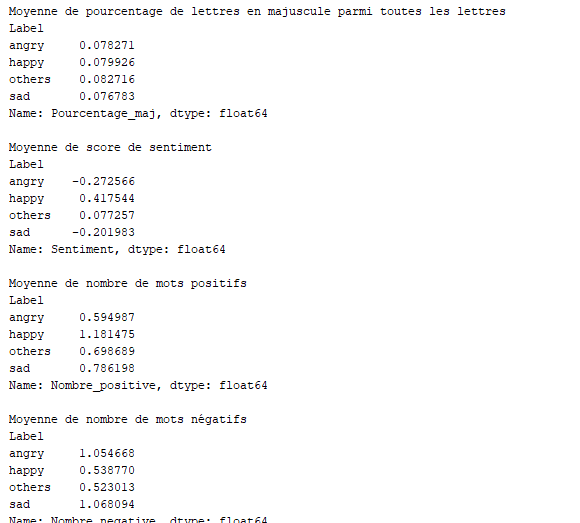
\includegraphics[width=\linewidth,height=15cm,keepaspectratio]{images/analyse_maj_sentiment}

Le score de sentiment utilisé est calculé avec \emph{Senti Word Net} en sommant les valeurs de sentiment attribuées à chaque mot de l'échange de textos. Le nombre de mots positifs/négatifs est calculé en comptant le nombre de mots avec des valeurs de sentiment supérieur/inférieur à 0.

On constate que le pourcentage de lettre majuscule dans les textos est similaire pour toutes les classes, on aurait pu penser qu'il aurait été plus haut pour les textos fâchés. 

Les 3 variables associées aux sentiments semblent beaucoup parler. En effet, les catégories triste et fâché ont des connotations beaucoup plus négatives, alors que la classe joyeuse a beaucoup plus de mots positifs. Cela n'est pas très surprenant.